\documentclass{if-beamer}

% --------------------------------------------------- %
%                  Presentation info	              %
% --------------------------------------------------- %

\title[Human Activity Recognition from Accelerometer Data]{Human Activity Recognition from Accelerometer Data}

\author[J. M. Yao]{\large{J. M. Yao}}

\institute[FRIBL/MSU]{FRIBL/NSCL, Michigan State University, East Lansing, Michigan 48824, USA
 }
\date{\today}
\logo{

\includegraphics[scale=0.15]{./figs/frib-logo.jpg}
}
\subject{Presentation subject} % metadata

\graphicspath{{figs/}}

 % --------------------------------------------------- %
%                    Title + Schedule                 %
% --------------------------------------------------- %

\begin{document}




  \begin{frame}
  \titlepage
\end{frame}


%\begin{frame}{Outline}
%  \tableofcontents
%\end{frame}

% --------------------------------------------------- %
%                      Presentation                   %
% --------------------------------------------------- %

\section{Introduction}



\begin{frame}{Introduction to the problem and dataset}

        \begin{block}{Seven activities (Challenge as not mutually exclusive)}
                            \begin{enumerate}
                            \item Working at Computer
                            \item Standing Up, \emph{Walking } and \exemple{Going Up/Downstairs}
                            \item  \alert{Standing}
                            \item \emph{Walking}
                            \item \exemple{Going Up/Down Stairs}
                            \item  \emph{Walking} and Talking with Someone
                            \item Talking while \alert{Standing}
                    \end{enumerate}
        \end{block}
        
        \begin{figure}
        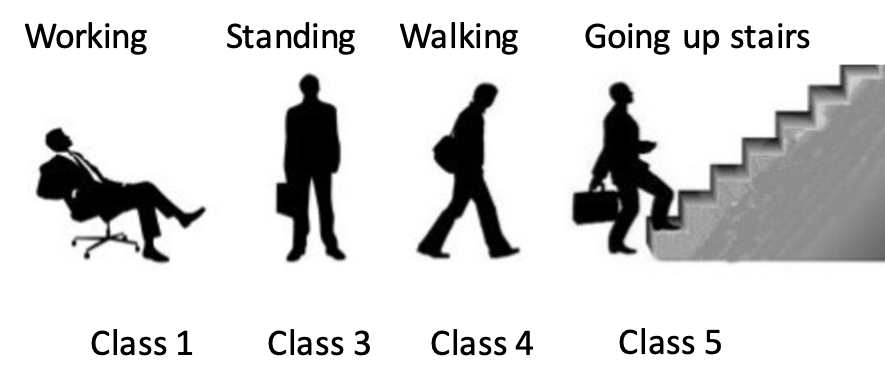
\includegraphics[scale=0.4]{./figs/activities.png}
        \end{figure}

\end{frame}


\begin{frame}{Introduction to the problem and dataset}
        \begin{block}{Task/Object: \emph{multi-class classification}}
                            \begin{itemize}
                            \item Input data:
                            
                                           \boxgrey{
                                            \centering
                                            \alert{Sequential number, x acceleration, y acceleration, z acceleration}
                                             } 
                                 
                            \item Output: 
                                             \boxgrey{
                                            \centering
                                            \alert{Class label ($1,2, \cdots, 7$) for each activity.}
                                             } 
                                 
                    \end{itemize}
        \end{block}
         
         
         \begin{block}{Procedure} 
                 \begin{figure}
        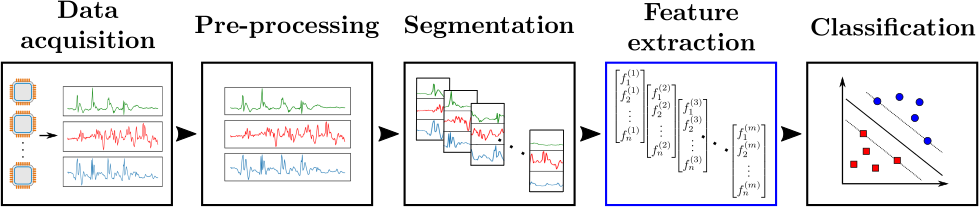
\includegraphics[scale=0.35]{./figs/process.png}
        \end{figure}
    \end{block}

\end{frame}




\section{Exploratory data analysis}

\begin{frame}{Exploratory data analysis: raw data}
        \begin{block}{An example data: participant 1}
                     \begin{figure}
                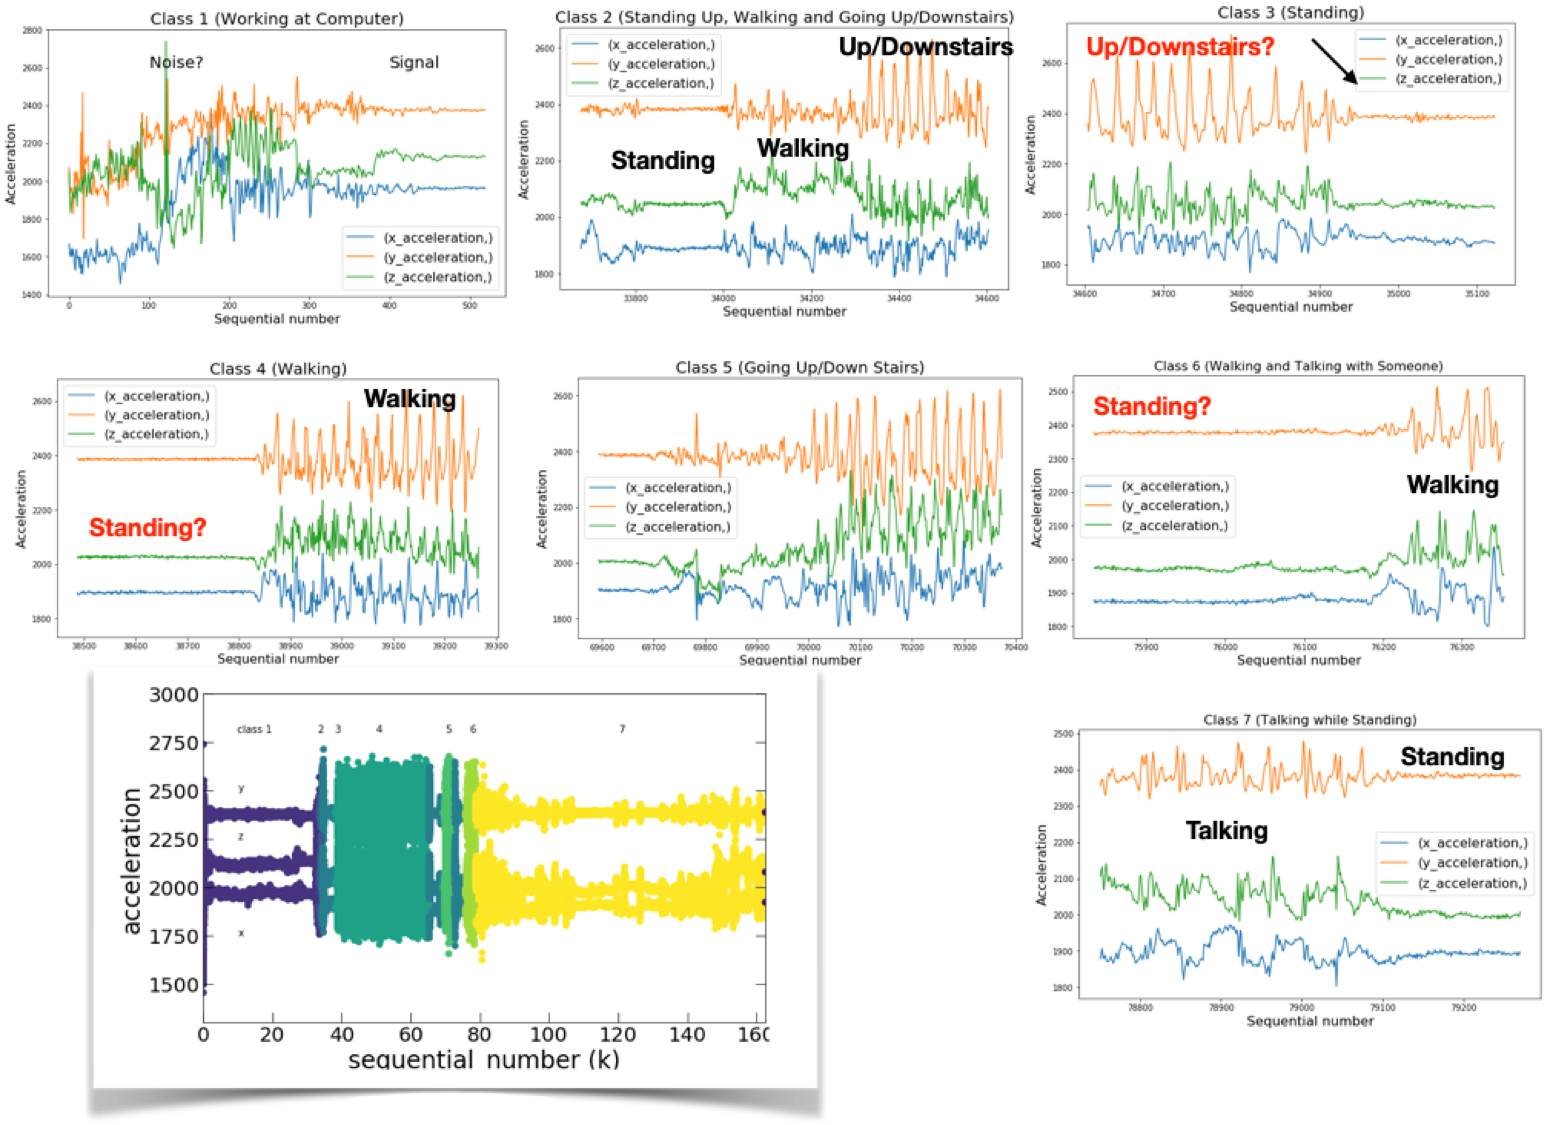
\includegraphics[scale=0.35]{./figs/paricipant01.png}
                \end{figure} 
   	 \end{block}
	
\end{frame}



\begin{frame}{Exploratory data analysis: raw data}


        \begin{block}{Feature extraction}
        
        \begin{itemize}
               \item  Generate samples/features using sliding temporal windows which split the raw data into segments. 
                
                \item The data (x, y, z-accelerations) in each window form one sample.  
         
             \item Hand-crafted features are extracted from each sample:
        \end{itemize}
        
        \begin{enumerate}
        		\item[$-$] \emph{Time domain features}: related to the distribution of the data
		
		 		 \boxgrey{ 
                                           mean $\mu_{i=x,y,z}$, variance $\sigma^2_i$, min, max, mean absolute deviation, skewness,
                                            kurtosis, correlation $Corr(i,j)$,  magnitude $\sqrt{\mu^2_x +  \mu^2_y + \mu^2_z}$
                                            }
                                            
                                            
 		\item[$-$]  \emph{Frequency domain features}:  energy-weighted moments:
			  
                            \begin{equation}
                            		M^{(k)} = \int d\omega \cdot \omega^k \cdot F(\omega),\quad k=1, 2, 3
                            \end{equation}
                            
                             where $F(\omega)$ is computed with Fast Fourier Transform (FFT)
                              \begin{equation}
                              		F(\omega) = \int dt \cdot f(t) \cdot e^{-i(2\pi\omega) t}.
                                \end{equation}


               \end{enumerate}
   	 \end{block}
	 
\end{frame}




\begin{frame}{Exploratory data analysis: raw data}
        \begin{block}{Fast Fourier Transformation (FFT)}
        \begin{equation}
        	X_k = \sum_{n=0}^{N-1} x_n e^{-i2\pi k n/N}  \qquad k = 0,\dots,N-1 
       \end{equation}         
        \begin{itemize}
         \item Compute the discrete Fourier transform of a sequence
         \item Computation complexity $O(n\log(n))$ (divide and conquer algorithm)
         \end{itemize}
         
         \vspace{-0.25cm}
         
               \begin{figure}
                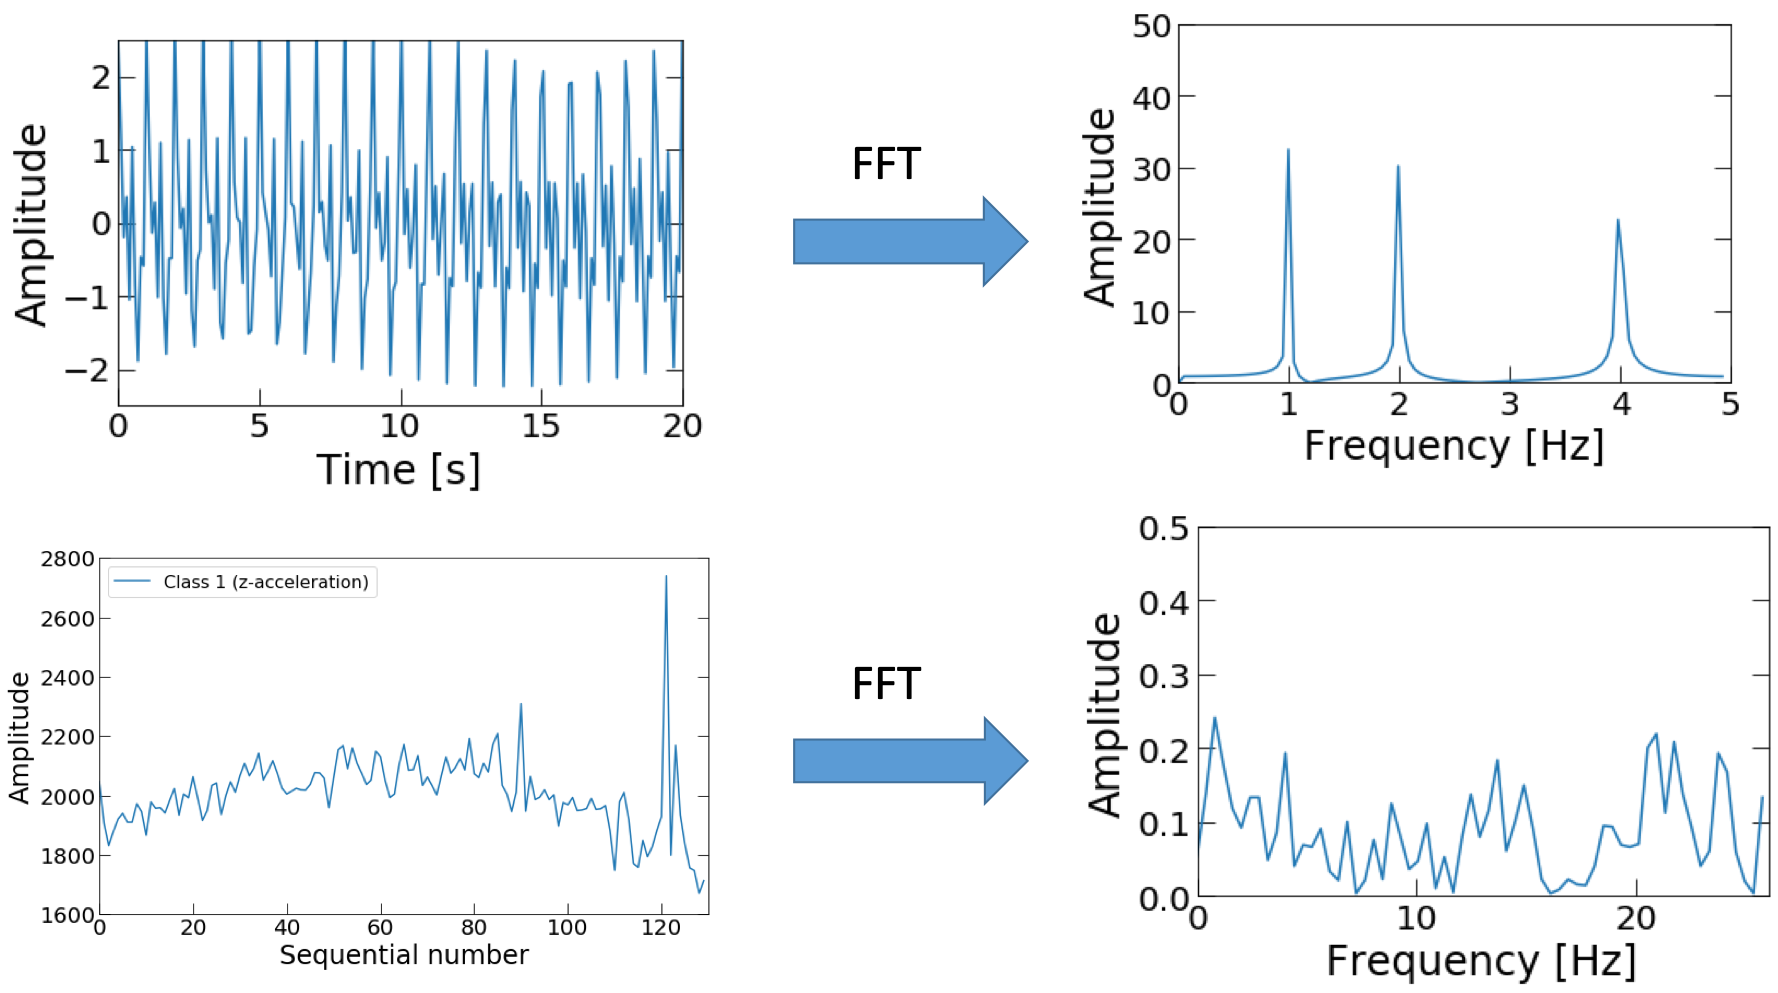
\includegraphics[scale=0.25]{./figs/FFT.png}
                \end{figure} 
   	 \end{block}
	
\end{frame}


\begin{frame}{Exploratory data analysis: sample data}
        \begin{block}{Imbalanced data}    
        \begin{itemize}
                \item Multi-class classification with imbalanced data is challenge. 
                \item Use a class dependent temporal window size.
                \item \alert{Risk of using window size information into training models}
        \end{itemize}                 
        
            	 \begin{figure}
                    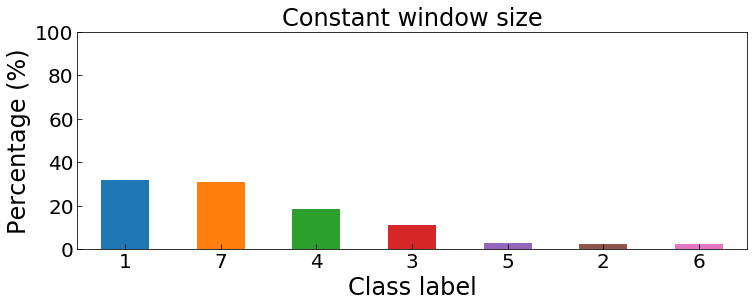
\includegraphics[scale=0.18]{./figs/percentage_origin.png}
                    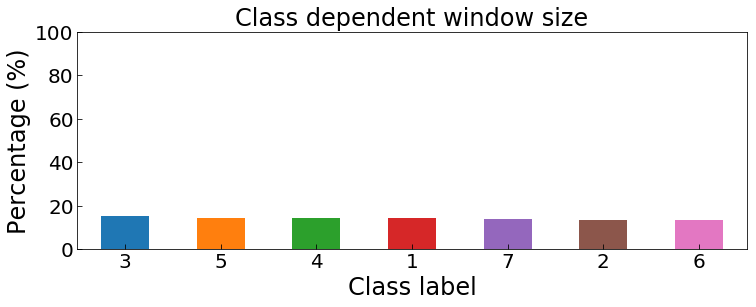
\includegraphics[scale=0.18]{./figs/percentage_balanced.png} 
                    \end{figure} 
   	 \end{block}
	
\end{frame}


 
\begin{frame}{Exploratory data analysis: sample data}
        \begin{block}{t-distributed Stochastic Neighbor Embedding (t-SNE)}    
        \begin{itemize}
                \item reduces dimensionality, trying to keep similar (dissimilar) instances close  (apart)
                \item tool for visualizing clusters of instances 
        \end{itemize}                 

         \begin{exampleblock}{Data with \emph{34} features}
            	 \begin{figure}
                    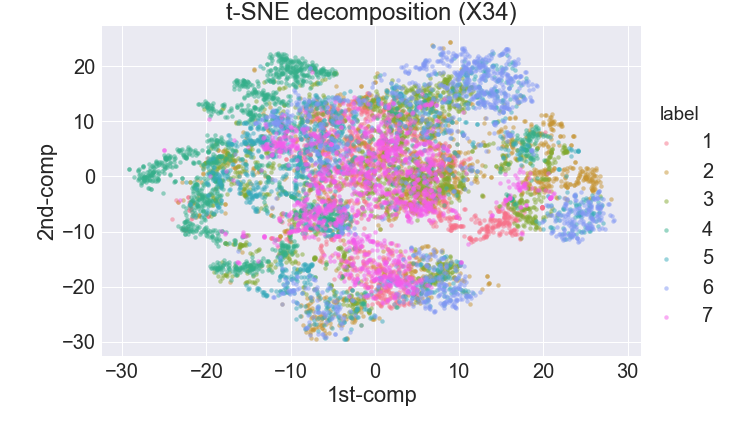
\includegraphics[scale=0.2]{./figs/tSNE12.png}
                    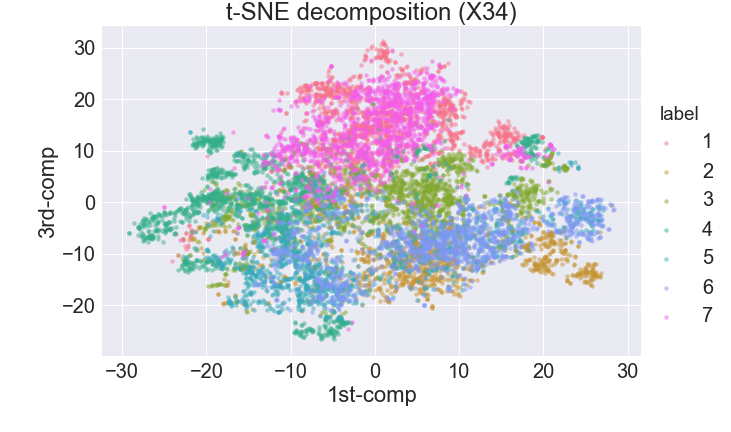
\includegraphics[scale=0.2]{./figs/tSNE13.png}
                    \end{figure} 
               \end{exampleblock}

   	 \end{block}
	
\end{frame}

\begin{frame}{Exploratory data analysis: sample data}

        \begin{block}{t-distributed Stochastic Neighbor Embedding (t-SNE)}    
        \begin{itemize}
                \item reduces dimensionality, trying to keep similar (dissimilar) instances close  (apart)
                \item tool for visualizing clusters of instances 
        \end{itemize}                 
        
         \begin{exampleblock}{Data with \emph{25} features (without \emph{frequency domain features)}}
            	 \begin{figure}
                    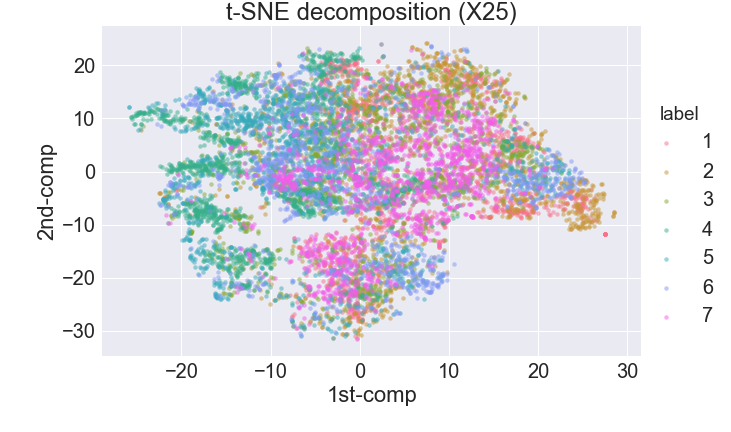
\includegraphics[scale=0.2]{./figs/tSNE12_X25.png}
                    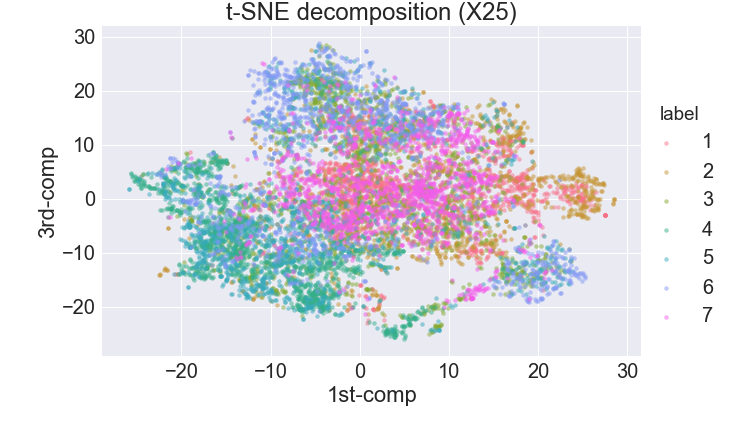
\includegraphics[scale=0.2]{./figs/tSNE13_X25.png}
                    \end{figure} 
               \end{exampleblock}
   	 \end{block}
	
\end{frame}
 





\section{Models}
 
 
 
\begin{frame}{Models}
\begin{columns}

 \begin{column}{0.5\textwidth}
    \begin{block}{Random Forest}
        \begin{itemize}
         \item non-parametric model
          \item \emph{provide importance of features}
         \item prone to overfitting
           \item regularization and monitoring train/test scores
        \end{itemize}
   \end{block} 
   
    \begin{exampleblock}{Confusion matrix (Test Data)}
      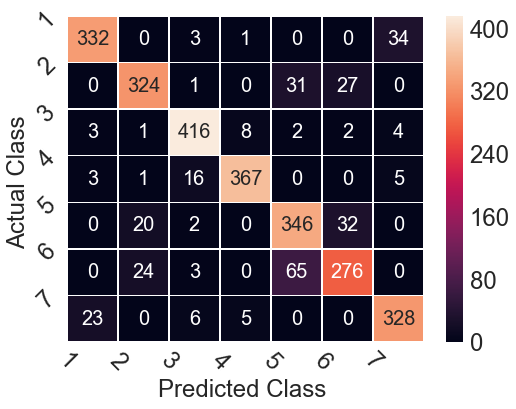
\includegraphics[scale=0.2]{./figs/rf_cm_default_X34.png}
      \end{exampleblock}

 \end{column}
  
\begin{column}{0.5\textwidth}


    Training the model with default parameters
       \begin{figure}
            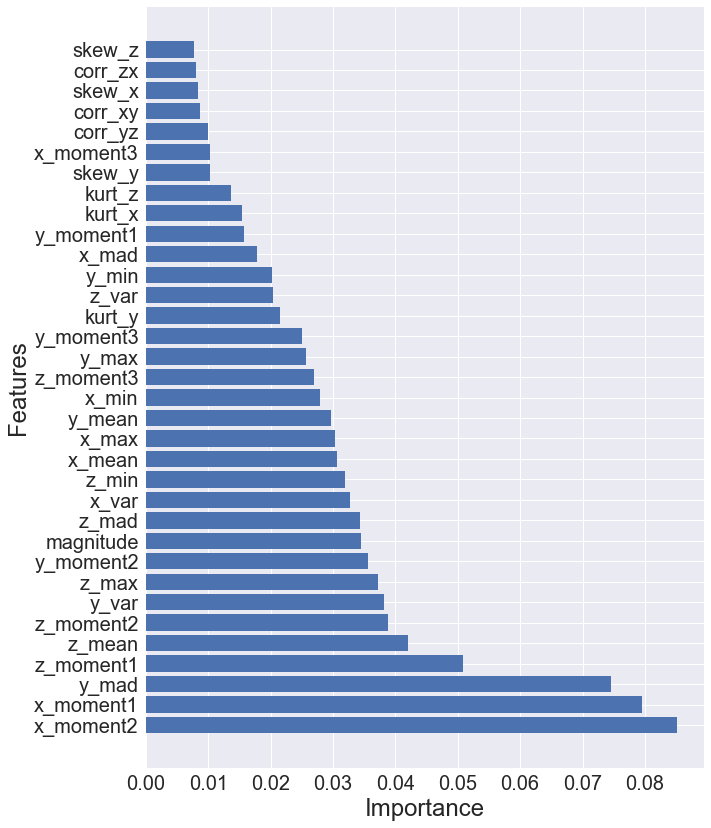
\includegraphics[scale=0.2]{./figs/importance.png}
            \end{figure}             
 \end{column}
 \end{columns}
\end{frame}

 
\begin{frame}{Models}
\begin{columns}

 \begin{column}{0.5\textwidth}
    \begin{block}{Random Forest}
        \begin{itemize}
         \item non-parametric model
          \item provide importance of features
         \item \emph{prone to overfitting} 
           \item regularization and monitoring train/test scores
        \end{itemize}
   \end{block} 
    \begin{exampleblock}{Confusion matrix (Test Data)}
      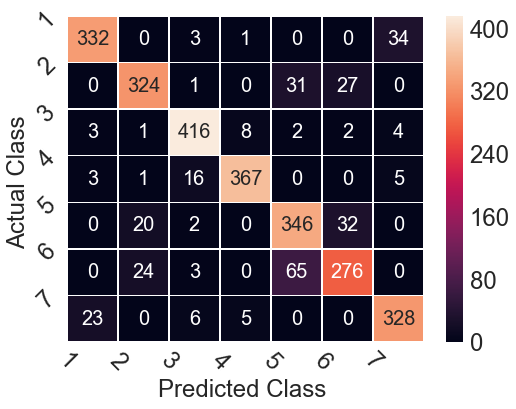
\includegraphics[scale=0.2]{./figs/rf_cm_default_X34.png}
      \end{exampleblock}
 \end{column}
  
\begin{column}{0.5\textwidth}


    Training the model with default parameters 
    
      \begin{figure}
            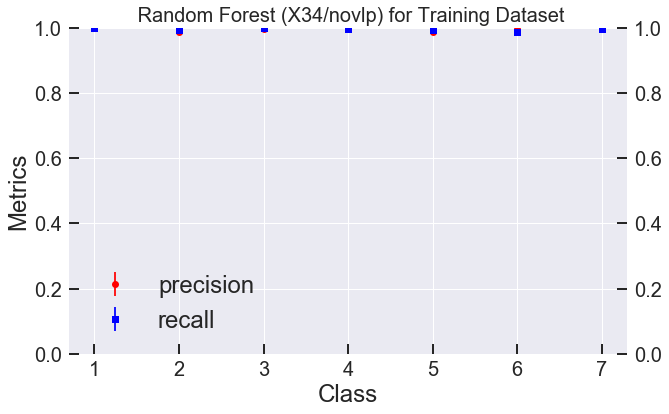
\includegraphics[scale=0.2]{./figs/rf_X34_train_default_score.png}
            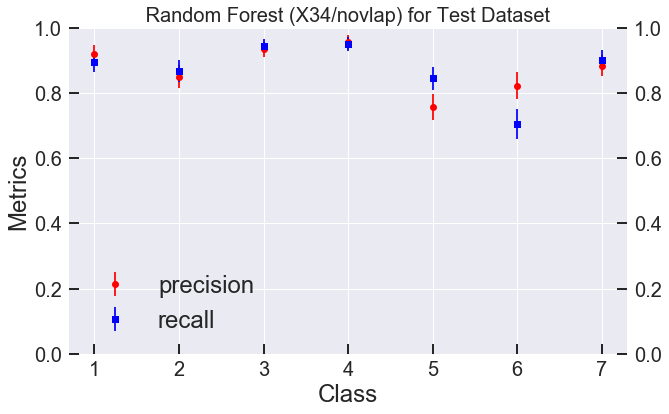
\includegraphics[scale=0.2]{./figs/rf_X34_test_default_score.png}
            \end{figure} 
            
 \end{column}
 \end{columns}
\end{frame}



 
  



\begin{frame}{Models}

\begin{columns}

 \begin{column}{0.5\textwidth}
    \begin{block}{Random Forest}
        \begin{itemize}
         \item non-parametric model
          \item provide importance of features
          \item prone to overfitting
           \item \emph{regularization and monitoring train/test scores}
        \end{itemize}
   \end{block}
   
    \begin{exampleblock}{GridSearch for the parameters}
     Introduce a new metric to take care of overfitting:
           \begin{equation}
          F_1 \equiv  f_1 ({\rm test}) - \emph{1.5}  \vert f_1 ({\rm train}) - f_1 ({\rm test}) \vert \nonumber
           \end{equation}
           where the $f_1$ measure is defined as
           \begin{equation}
           f_1 = \dfrac{2}{\dfrac{1}{precision} + \dfrac{1}{recall}} 
           \end{equation}
   \end{exampleblock}
    
 \end{column} 
\begin{column}{0.5\textwidth}
  Training the model with GridSearch  
             \begin{figure}
            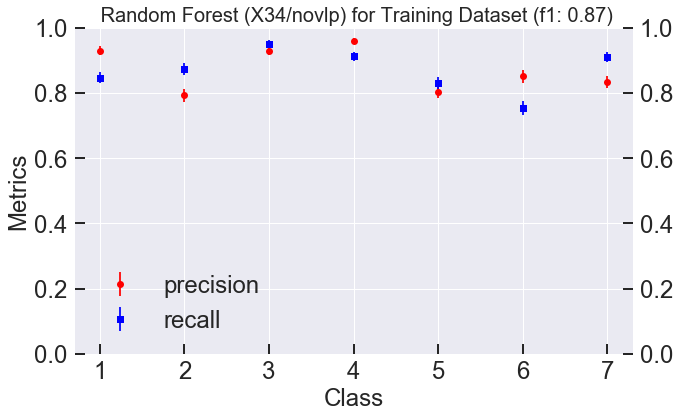
\includegraphics[scale=0.2]{./figs/rf_X34_train_score.png}
            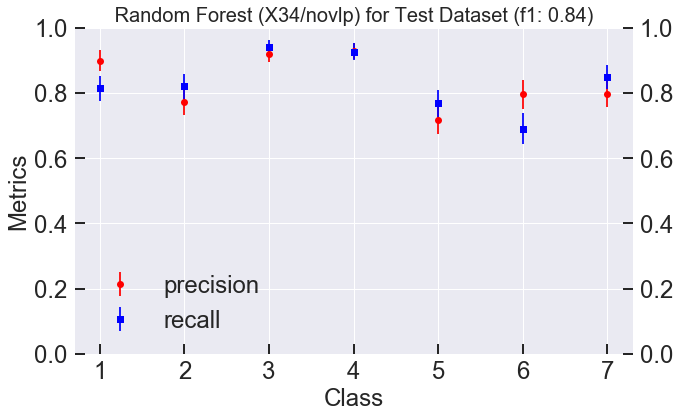
\includegraphics[scale=0.2]{./figs/rf_X34_test_score.png}
            \end{figure}
 \end{column}
 \end{columns}
\end{frame}


\begin{frame}{Models: overlapping windows or not} 
    
    \begin{columns}
   \begin{column}{0.5\textwidth} 
                \boxblue{
                \centering 
                Non-overlapping windows}

            \begin{figure}
            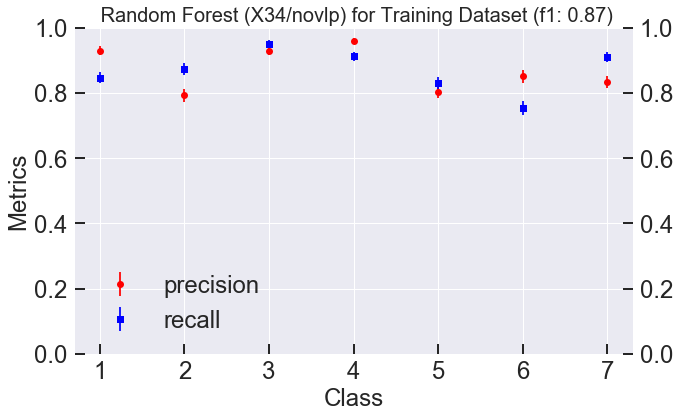
\includegraphics[scale=0.2]{./figs/rf_X34_train_score.png}
            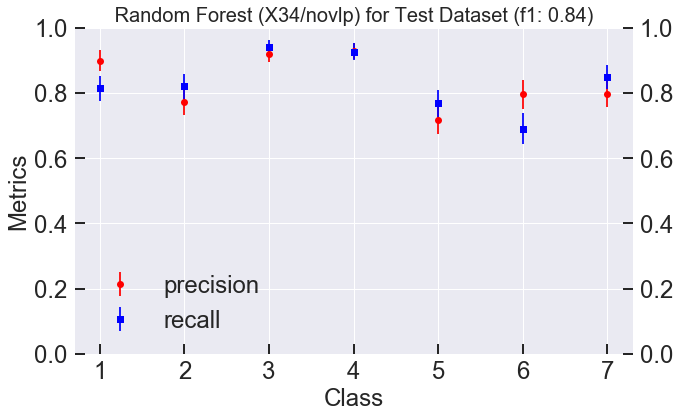
\includegraphics[scale=0.2]{./figs/rf_X34_test_score.png}
            \end{figure}
   \end{column} 
    
\begin{column}{0.5\textwidth}

                \boxblue{
                \centering 
                Half-overlapping windows}
             \begin{figure}
            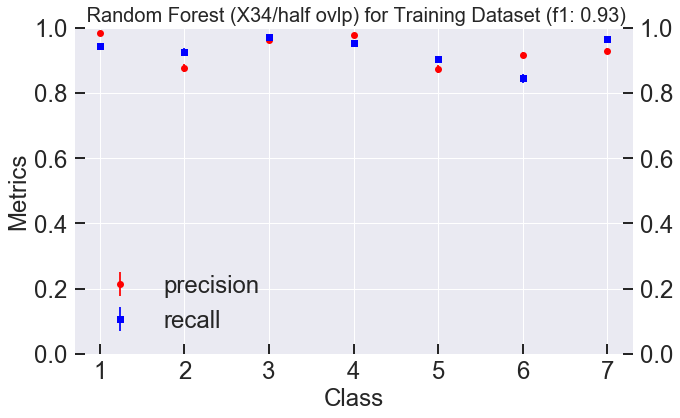
\includegraphics[scale=0.2]{./figs/rf_X34_half_train_score.png}
            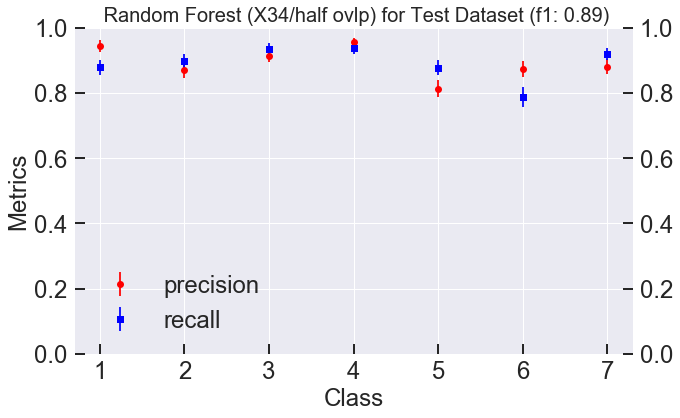
\includegraphics[scale=0.2]{./figs/rf_X34_half_test_score.png}
            \end{figure}
            
 \end{column}

 \end{columns}
\end{frame}



\begin{frame}{Models: with frequency domain features or not} 
    
    \begin{columns}
   \begin{column}{0.5\textwidth} 
                \boxblue{
                \centering 
                w/o frequency domain features}

            \begin{figure}
            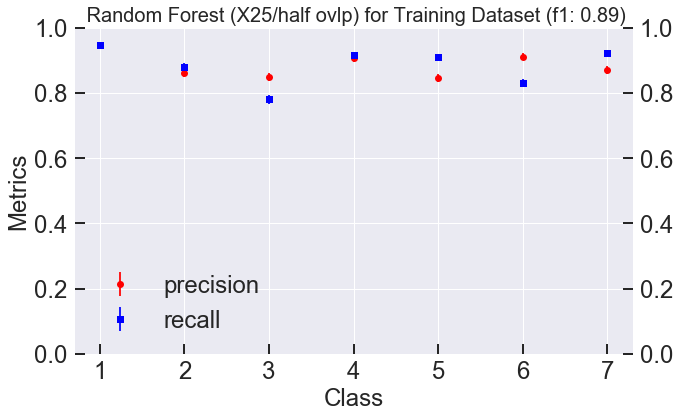
\includegraphics[scale=0.2]{./figs/rf_X25_half_train_score.png}
            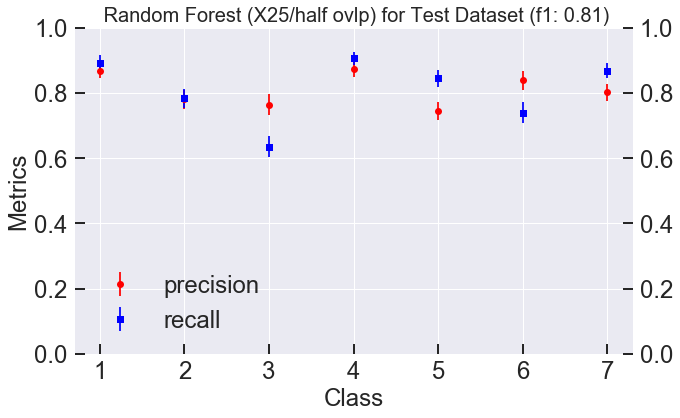
\includegraphics[scale=0.2]{./figs/rf_X25_half_test_score.png}
            \end{figure}
   \end{column} 
    
\begin{column}{0.5\textwidth}

                \boxblue{
                \centering 
                w/ frequency domain features}
             \begin{figure}
            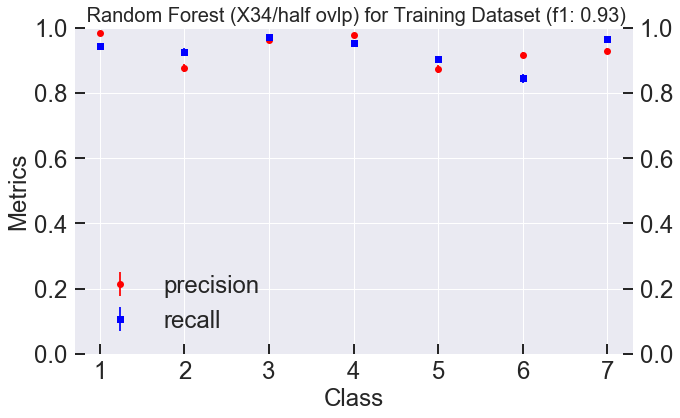
\includegraphics[scale=0.2]{./figs/rf_X34_half_train_score.png}
            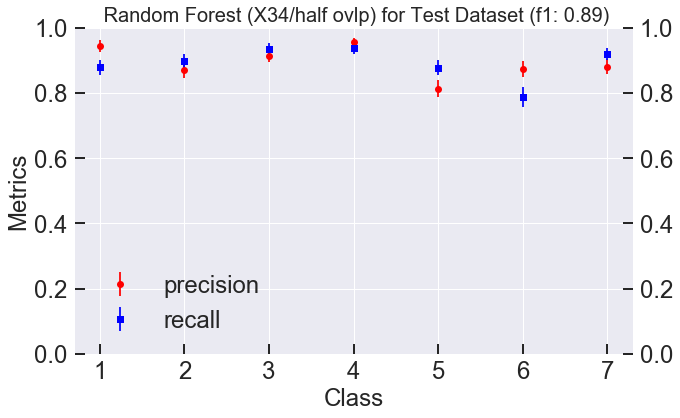
\includegraphics[scale=0.2]{./figs/rf_X34_half_test_score.png}
            \end{figure}
            
 \end{column}

 \end{columns}
 
\end{frame}
 





\begin{frame}{Models: window size effect} 
    \begin{exampleblock}{Precision/Recall for test data in the Random Forest}
             \begin{figure}
            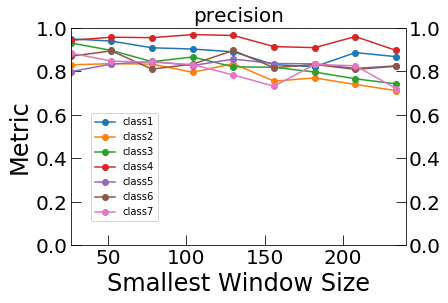
\includegraphics[scale=0.3]{./figs/Precision_Test_Ovlp_Window_Size.png}
            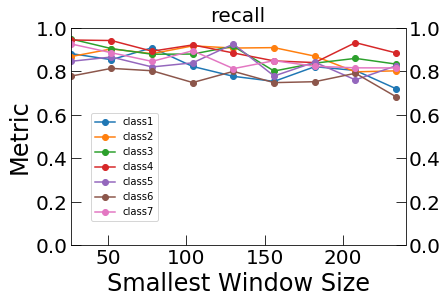
\includegraphics[scale=0.3]{./figs/Recall_Test_Ovlp_Window_Size.png}
            \end{figure}
        \end{exampleblock}      
        
        \begin{itemize}
        \item Globally, the score is slightly decreasing with the window size.
        \end{itemize}
        
   \end{frame}



\begin{frame}{Models:  KNeighborsClassifier (KNN)} 

    \begin{columns}
    
   \begin{column}{0.5\textwidth} 
   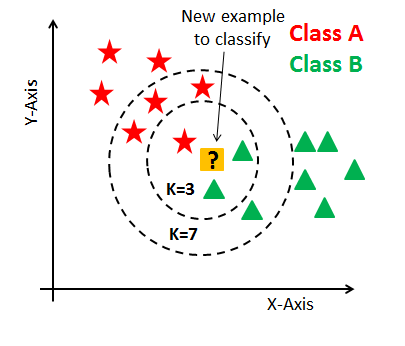
\includegraphics[scale=0.3]{./figs/KNN.png}
   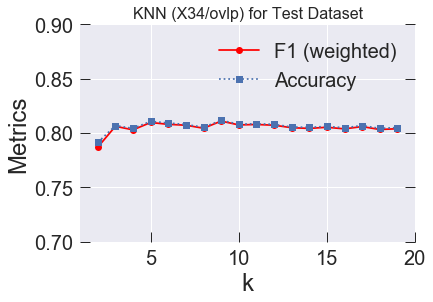
\includegraphics[scale=0.3]{./figs/knn_X34_half_test_score_k.png}

   \end{column} 
    
\begin{column}{0.5\textwidth}
 
             \begin{figure}
            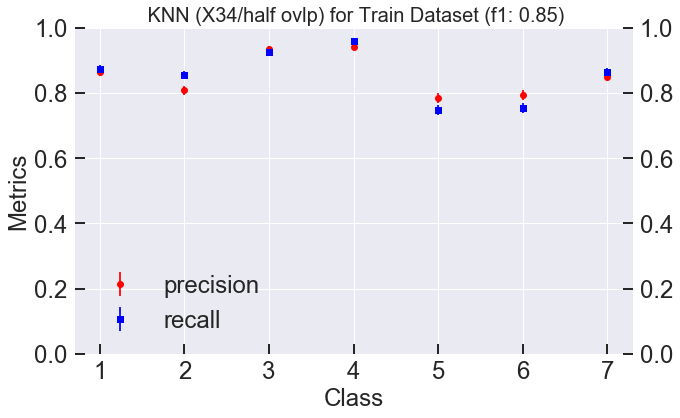
\includegraphics[scale=0.23]{./figs/knn_X34_half_train_score.png}
            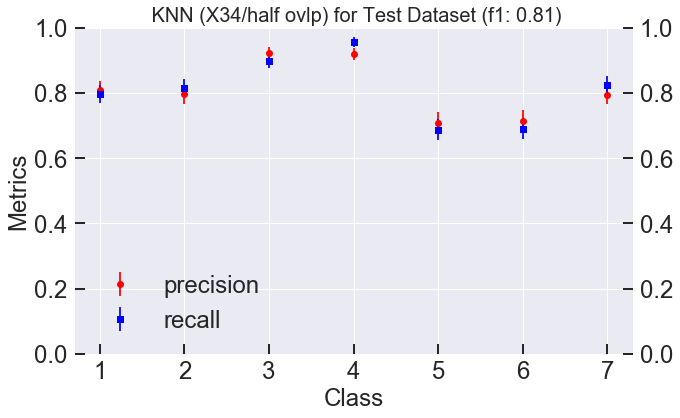
\includegraphics[scale=0.23]{./figs/knn_X34_half_test_score.png}
            \end{figure}  
        
 \end{column}

 \end{columns}
   \end{frame}


\begin{frame}{Models:  Support Vector Machine Classification (SVC)} 

    \begin{columns}
   \begin{column}{0.5\textwidth} 
   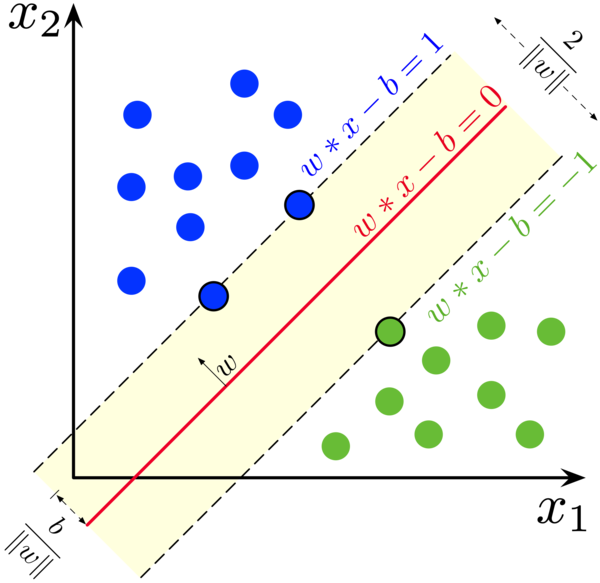
\includegraphics[scale=1]{./figs/svc.png} 
   
   \begin{itemize}
   \item kernel: radial basis function
           \begin{equation}
           	K(X_i, X_j) = \exp[-\gamma  (X_i - X_j)^2]
           \end{equation}
   \item decrease $\gamma$ to prevent overfitting
   \item decrease $C$ to prevent overfitting
   \end{itemize}

   \end{column} 
    
   \begin{column}{0.5\textwidth}
 
             \begin{figure}
            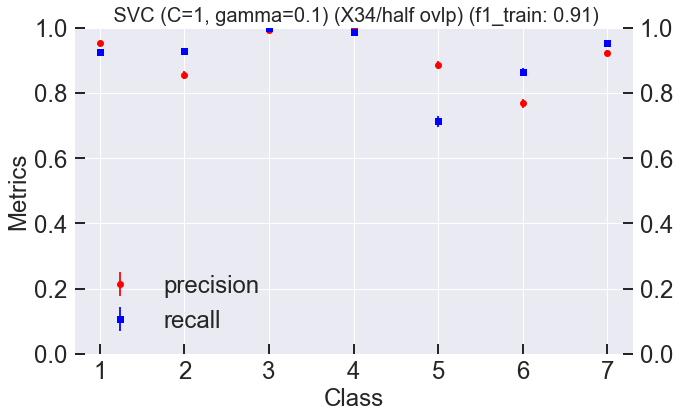
\includegraphics[scale=0.23]{./figs/svc_X34_half_train_score.png}
            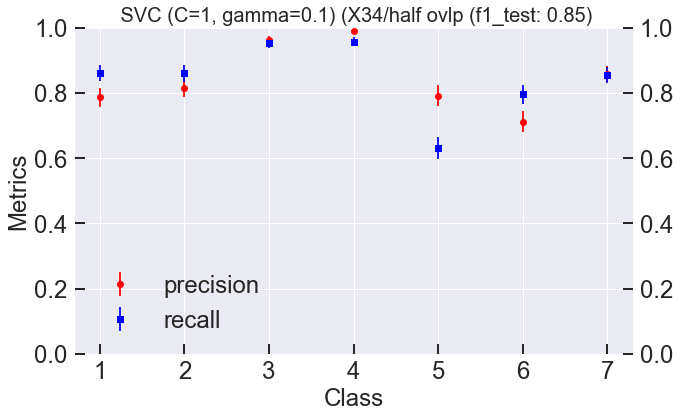
\includegraphics[scale=0.23]{./figs/svc_X34_half_test_score.png}
            \end{figure}  
        
 \end{column}

 \end{columns}
   \end{frame}




\begin{frame}{Models:  Ensemble methods} 

  \begin{columns}
   \begin{column}{0.5\textwidth} 
   \begin{exampleblock}{Voting}
   \begin{itemize}
   \item Use the pre-trained (optimized) SVC, KNN, and Random Forest algorithms
   \item Aggregate the predictions of each classifier and predict the class that gets the most votes
   \item Generally, better than each of the three algorithms
      \end{itemize}
      \end{exampleblock}
      
   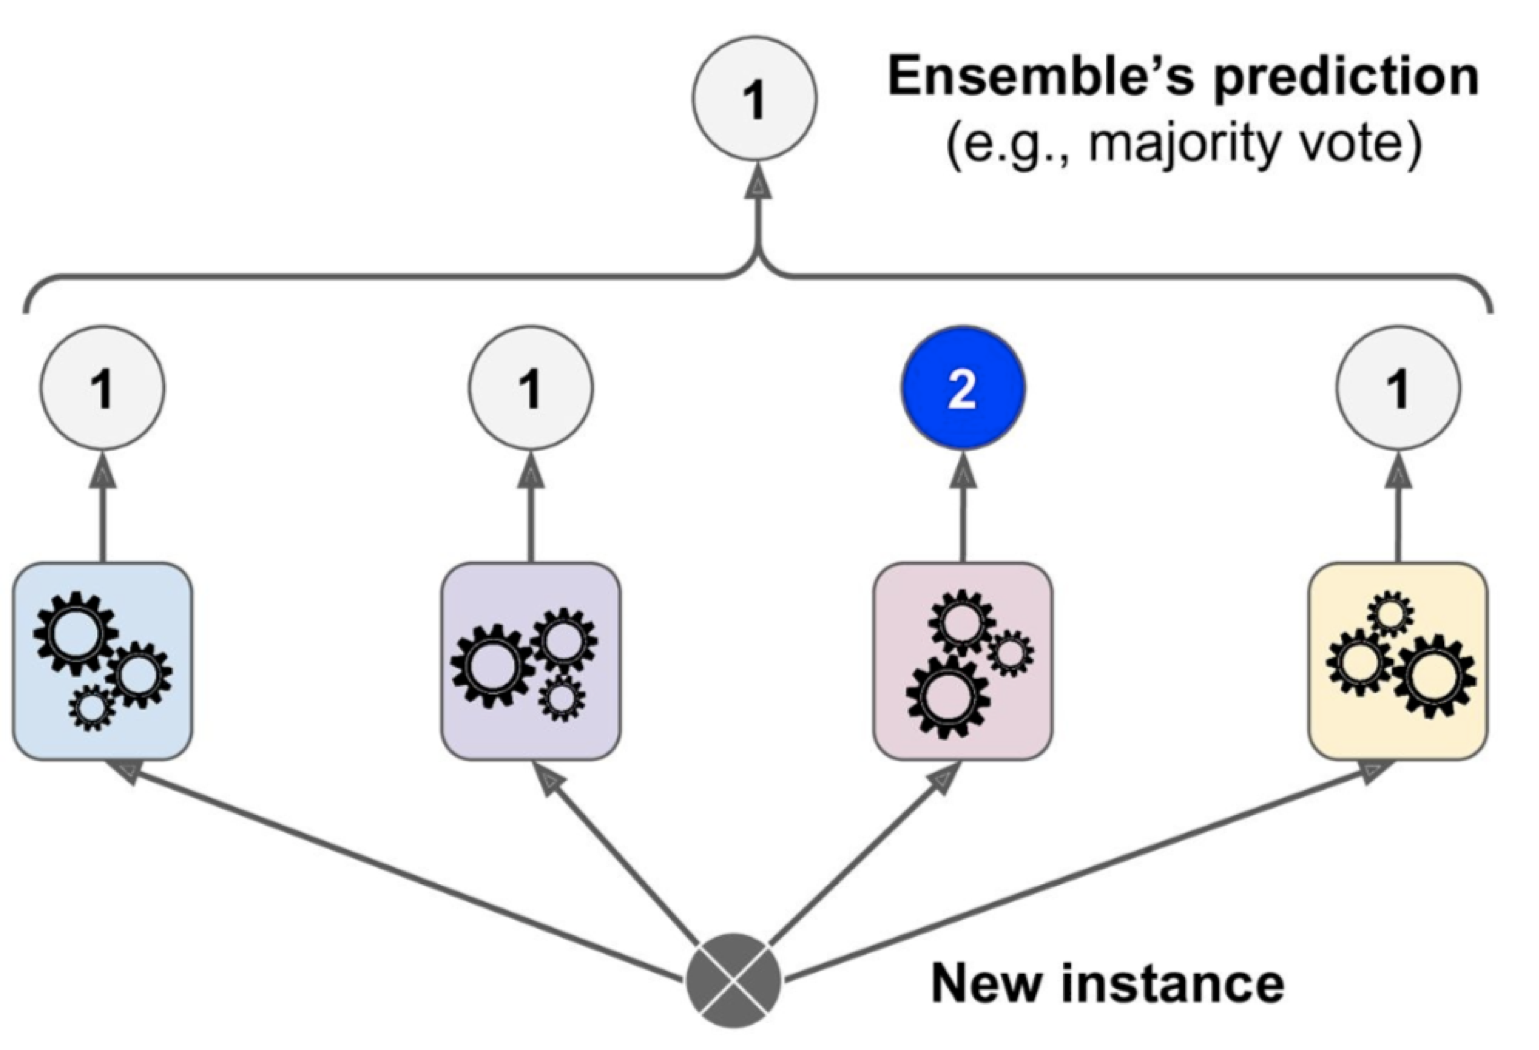
\includegraphics[scale=0.2]{./figs/voting.png} 

   \end{column} 
    
   \begin{column}{0.5\textwidth}
 
             \begin{figure}
            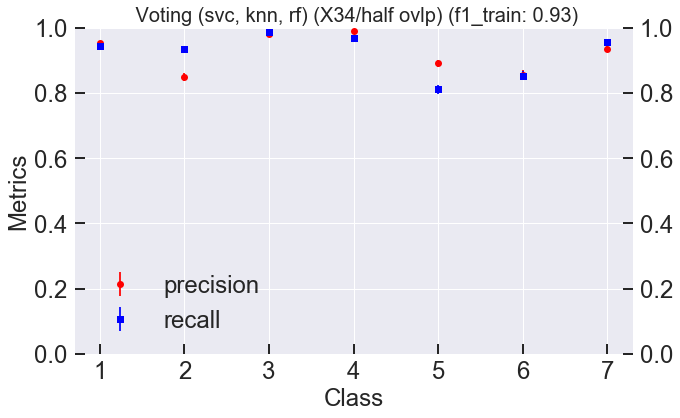
\includegraphics[scale=0.23]{./figs/voting_X34_train.png}
            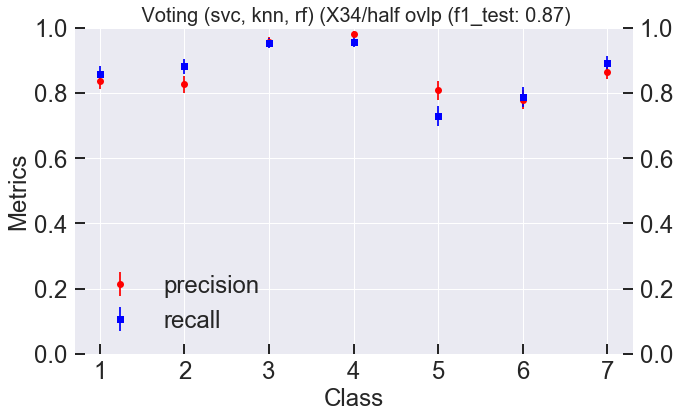
\includegraphics[scale=0.23]{./figs/voting_X34_test.png}
            \end{figure}  
        
 \end{column}

 \end{columns}
  \end{frame}



\begin{frame}{Models:  Ensemble methods} 

  \begin{columns}
   \begin{column}{0.5\textwidth} 
   \begin{exampleblock}{Bagging}
   \begin{itemize}
   
   \item  Use the pre-trained Random Forest classifier as the base classifier
   \item Fit the  base classifier to random 20 subsets of the original dataset (reduce variance)
      \end{itemize}
      \end{exampleblock}
      
   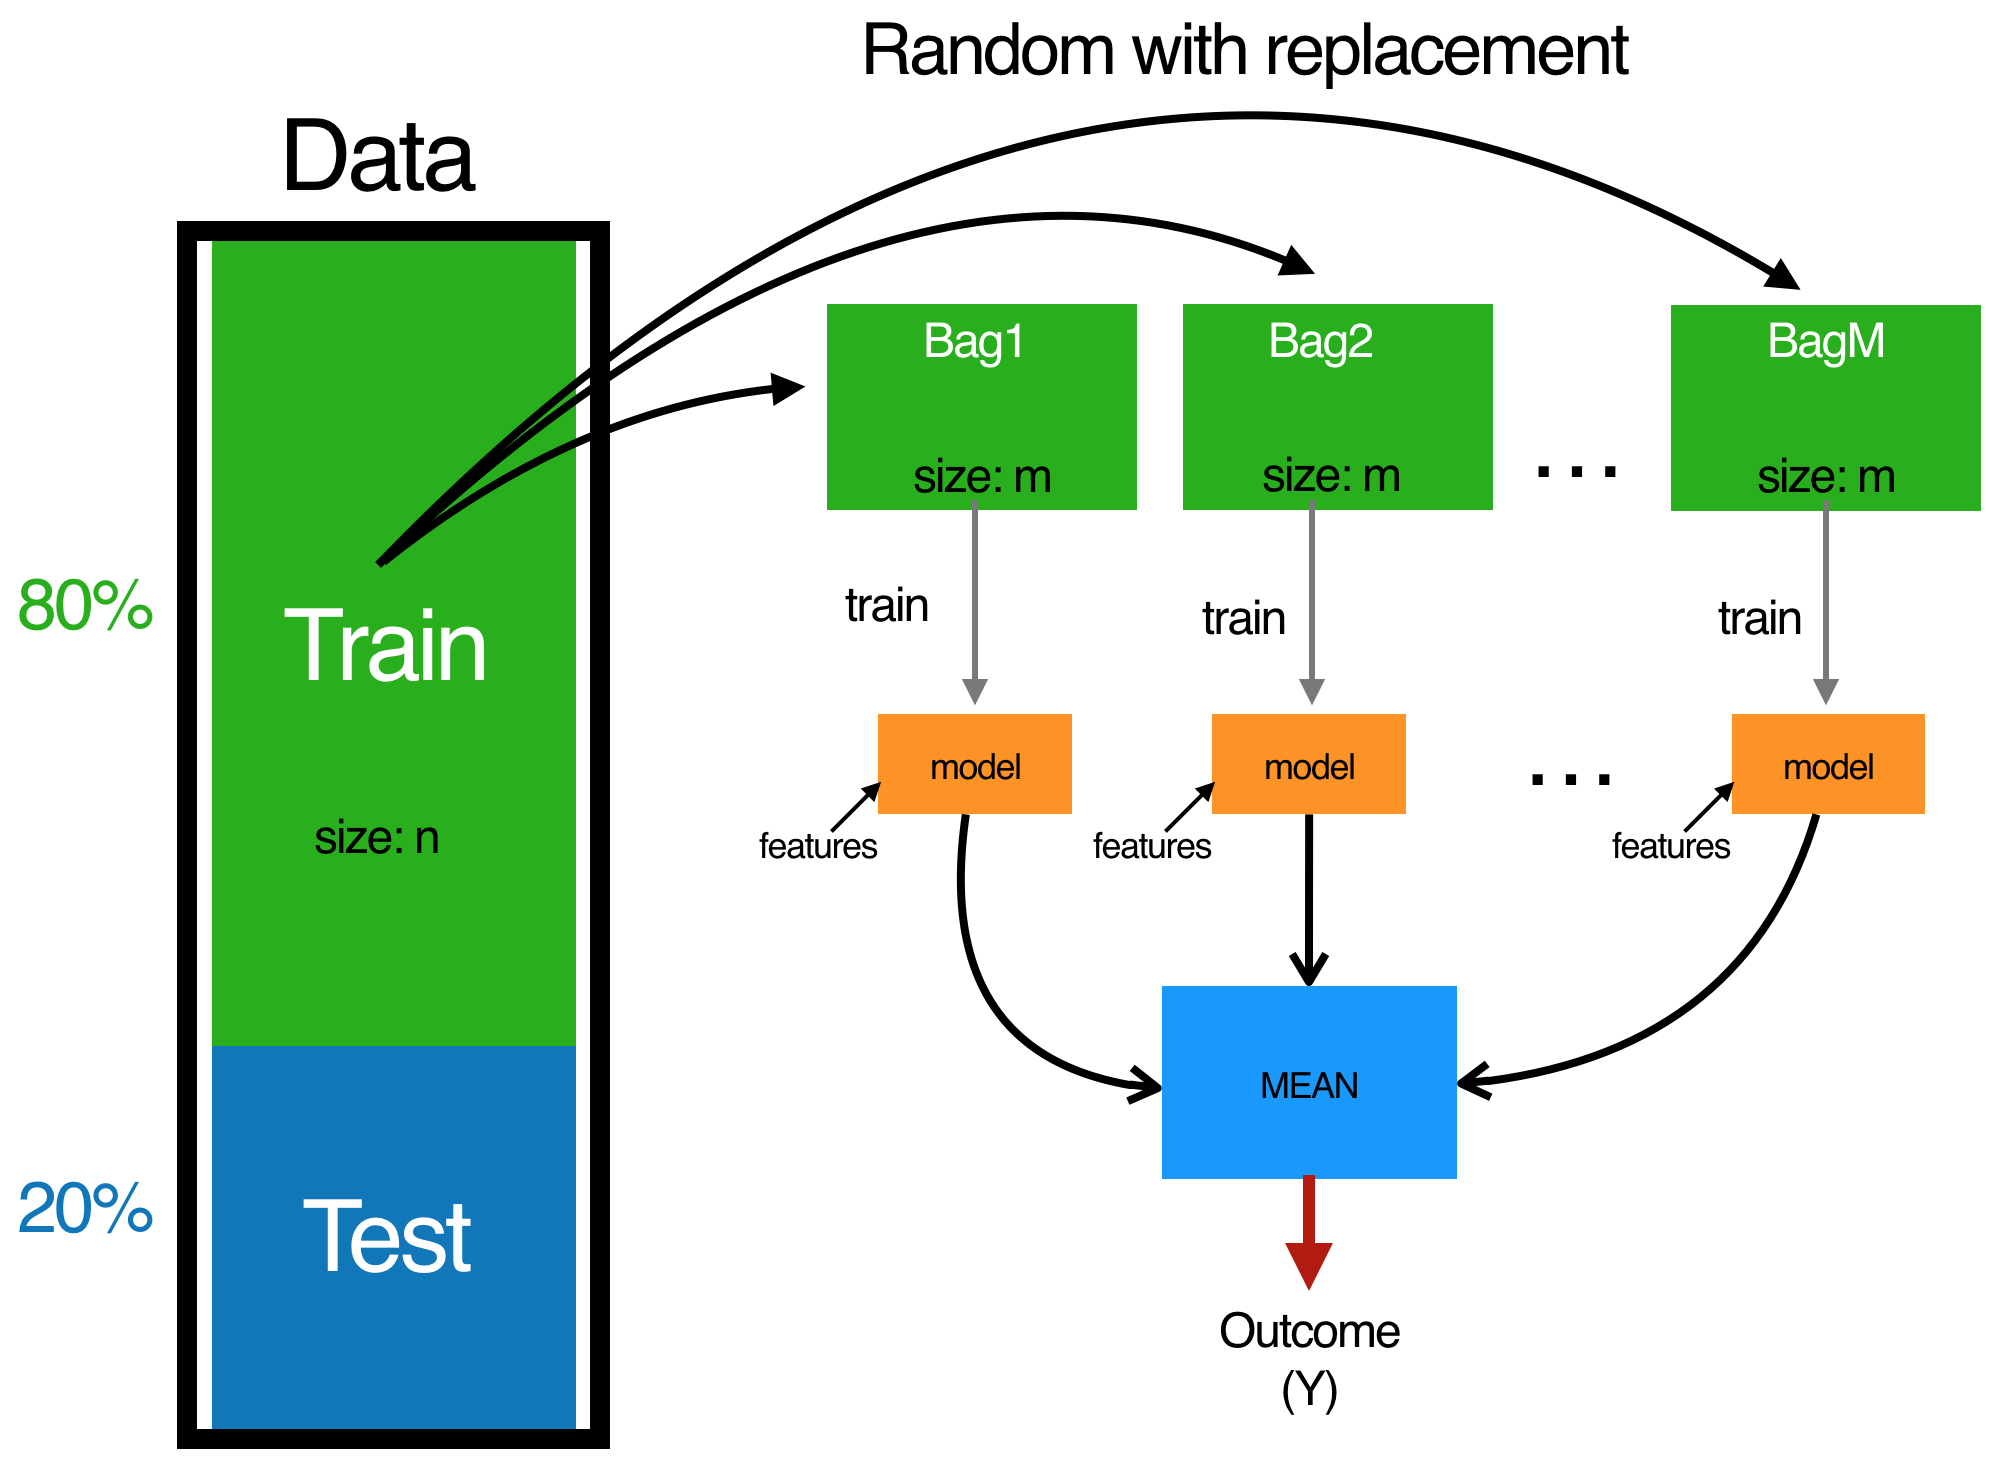
\includegraphics[scale=0.15]{./figs/bagging.png} 

   \end{column} 
    
   \begin{column}{0.5\textwidth}
 
             \begin{figure}
            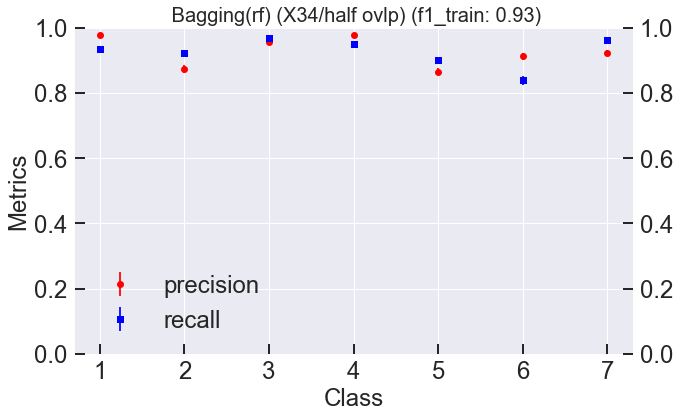
\includegraphics[scale=0.23]{./figs/bagging_X34_train.png}
            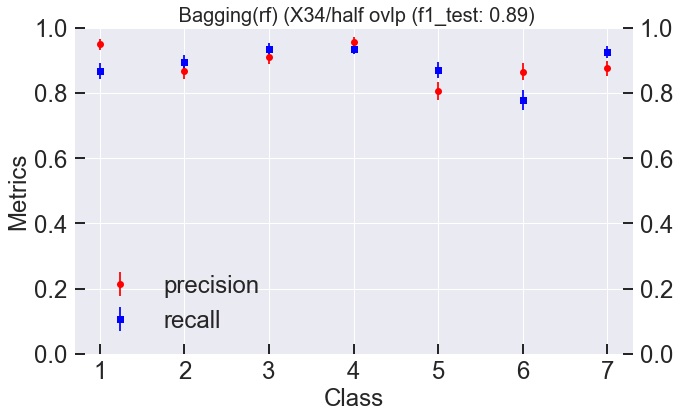
\includegraphics[scale=0.23]{./figs/bagging_X34_test.png}
            \end{figure}  
        
 \end{column}

 \end{columns}
  \end{frame}
  
  
  
  
\begin{frame}{Models:  Ensemble methods} 

  \begin{columns}
   \begin{column}{0.5\textwidth} 
   \begin{exampleblock}{XGBoost (eXtreme Gradient Boosting)}
   \begin{itemize}
   
   \item  Gradient boosted decision trees
   \item "state-of-the-art” machine learning algorithm for structured or tabular datasets on classification and regression
   (faster, wide variety of tuning parameters, better performance)
      \end{itemize}
      \end{exampleblock}
      
   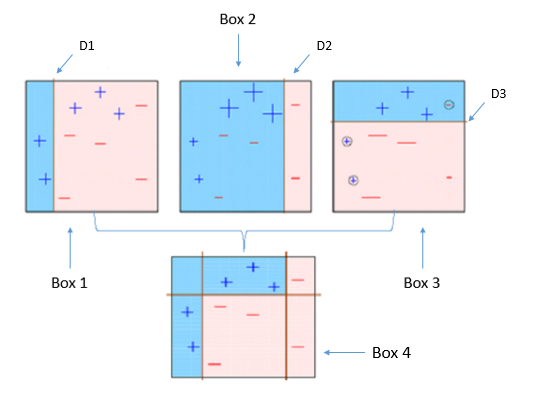
\includegraphics[scale=0.25]{./figs/boosting.png} 

   \end{column} 
    
   \begin{column}{0.5\textwidth}
 
             \begin{figure}
            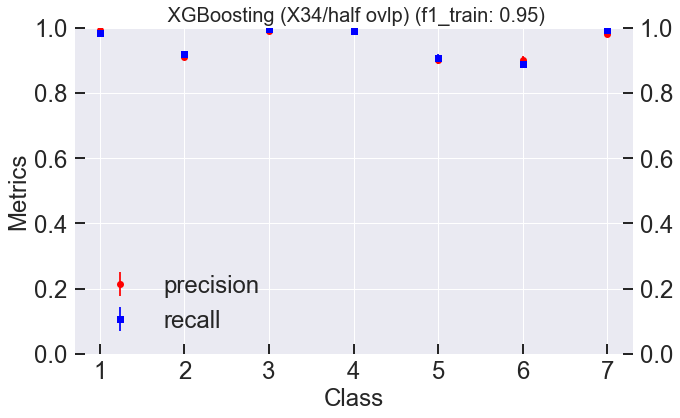
\includegraphics[scale=0.23]{./figs/xgb_X34_train.png}
            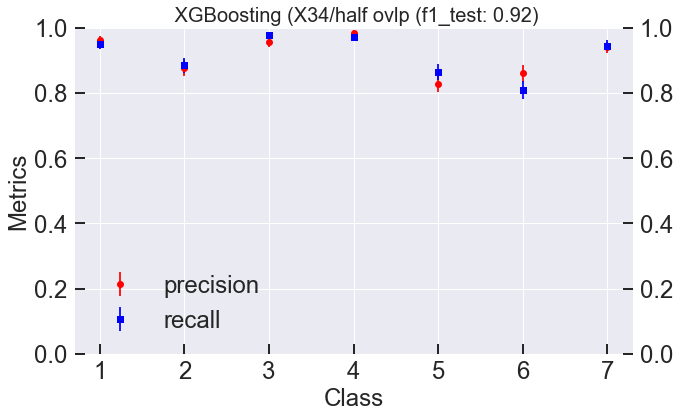
\includegraphics[scale=0.23]{./figs/xgb_X34_test.png}
            \end{figure}  
        
 \end{column}

 \end{columns}
  \end{frame}
  
  
\begin{frame}{Models:  comparison} 
  
    \begin{columns}
   \begin{column}{0.6\textwidth} 
             \begin{figure}
            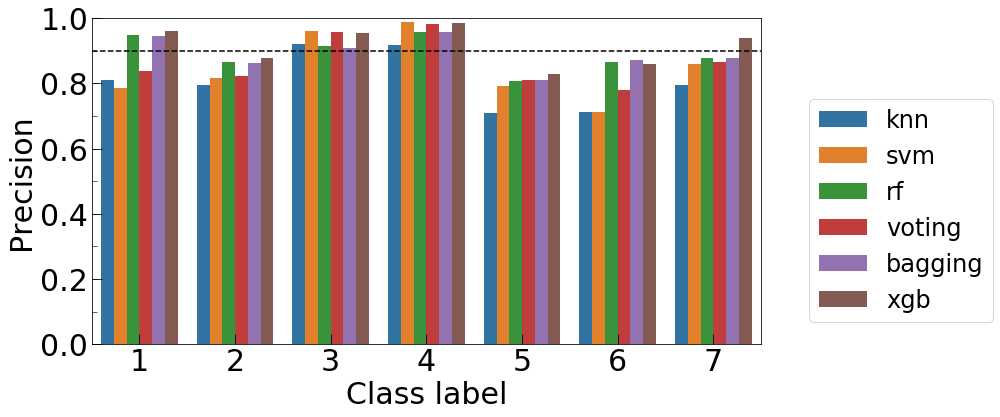
\includegraphics[scale=0.19]{./figs/comparison_precision.png}
            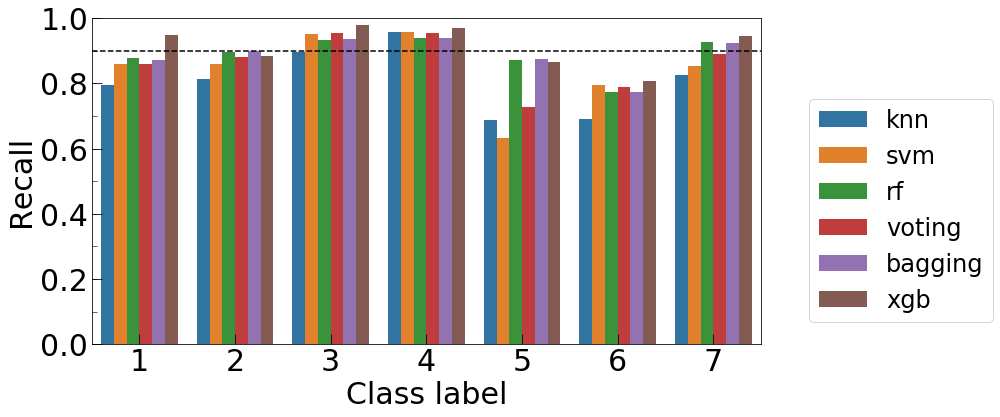
\includegraphics[scale=0.19]{./figs/comparison_recall.png}
            \end{figure}  


   \end{column} 
    
   \begin{column}{0.4\textwidth}
   
        \begin{block}{Activities}
                            \begin{enumerate}
                            \item Working at Computer
                            \item \emph{Standing Up, Walking  and Going Up/Downstairs}
                            \item  Standing
                            \item  Walking
                            \item \emph{Going Up/Down Stairs}
                            \item  \emph{Walking and Talking with Someone}
                            \item Talking while  Standing
                    \end{enumerate}
        \end{block}
        
                    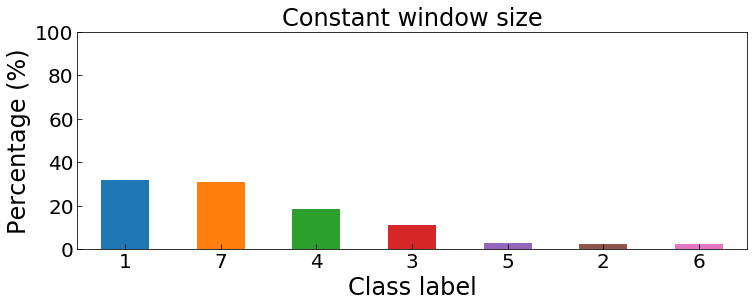
\includegraphics[scale=0.16]{./figs/percentage_origin.png}
        
        
 \end{column}

 \end{columns}


  \end{frame}
  
  \section{Summary and outlook}
  
\begin{frame}{Summary and outlook} 


    \begin{block}{Summary}
   \begin{itemize}
        \item Frequency domain features are very important 
        \item Using non-overlapping and half-overlapping sliding windows have a significant influence (leaking test data into the training data, larger sample size?) 
        \item Increase in  window size globally decreases the performance (sample size effect?)
        \item Balanced data are important in multi-class classification to have a similar performance on each class.
        \item XGBoost turns out to have the best performance among machine learning models
   
   \end{itemize}
  \end{block}
  
  \begin{exampleblock}{Outlook}
      \begin{itemize}
       \item Collect more data for the class 2, 5, and 6 
       \item Collect some information other than the acceleration along 3 directions (angles?)
       
       \item More detailed fine tunings on the model parameters          
       \item Deep learning models (CNN/RNN) are worth to try when the dataset is large enough
       \end{itemize}
  \end{exampleblock}
   
 
  \end{frame}
  
  
\begin{frame}{Acknowledgement}    
 
   \centering 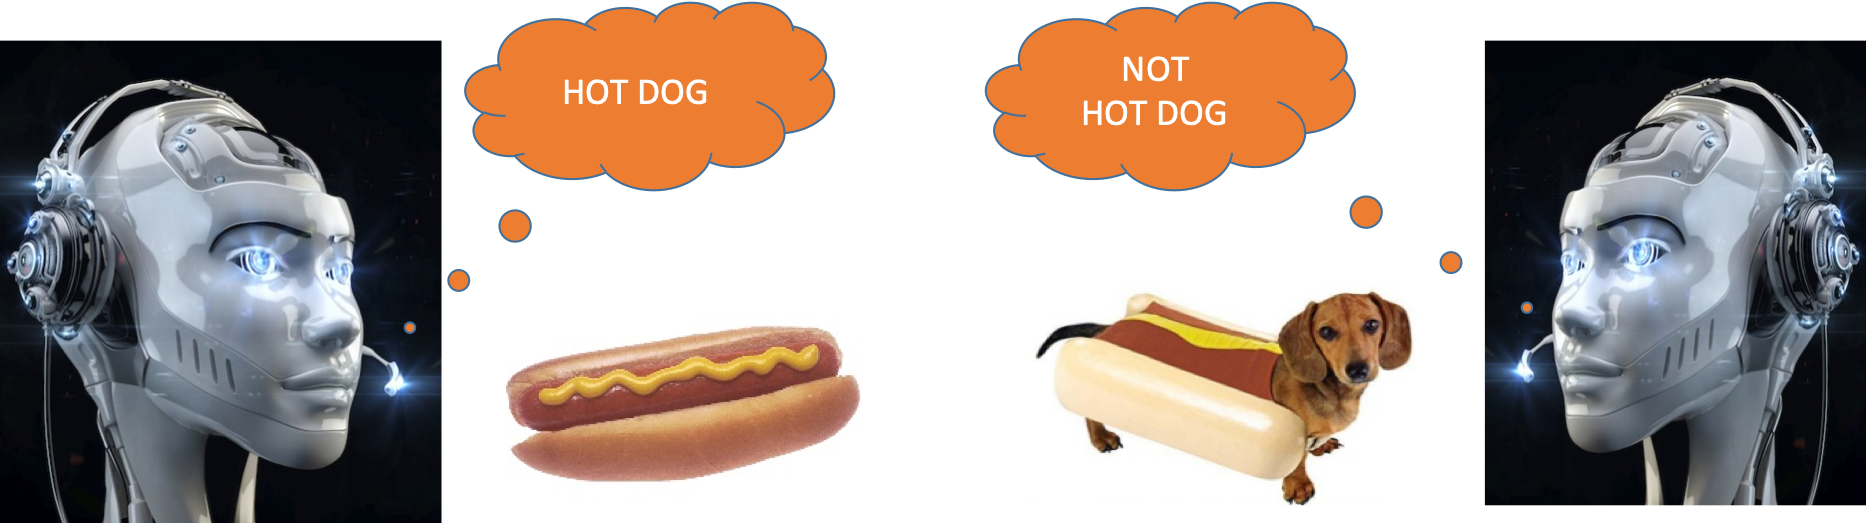
\includegraphics[scale=0.3]{./figs/hotdog.png}
 
\boxorange{ \centering Special thanks to Alexander Tolpygo from SFL Scientific for providing all the data for the project.}

  \centering  \Huge Thank you all for your attention !
 
  \end{frame}




   

\begin{frame}[fragile]
\frametitle{Code Example \#1}

%\code{\textbf{import} numpy \textbf{as} np}

 \begin{exampleblock}{XGBoost}
 
      \begin{lstlisting}[language=Python]
      def xgboost_fit_predict(X_train,y_train,X_test,y_test):
            xgb_reg = xgboost.XGBClassifier(n_estimators=1000, random_state=42)
            xgb_reg = xgb_reg.fit(X_train, y_train, eval_metric=["merror"],
                              eval_set=[[X_train, y_train],[X_test, y_test]],
                              verbose=100,
                              early_stopping_rounds=10)
            
            y_pred = xgb_reg.predict(X_test)
            val_error = mean_squared_error(y_test, y_pred)
            print("Validation MSE:", val_error) 
            
            
            y_pred4test        = xgb_reg.predict(X_test)
            y_pred4train       = xgb_reg.predict(X_train)
            
            xgb_clf_best_cm4test = metrics.confusion_matrix(y_test, y_pred4test)
            xgb_clf_best_cm4train = metrics.confusion_matrix(y_train, y_pred4train)
            
            print("F1 score for Test: {}".format(f1_score(y_test,y_pred4test, average='weighted')))
            print("F1 score for Train: {}".format(f1_score(y_train,y_pred4train, average='weighted'))) 
            
      \end{lstlisting}
 \end{exampleblock}


\end{frame}


  
\begin{frame}{XGBoost: merror in train and test}    
 
   \centering 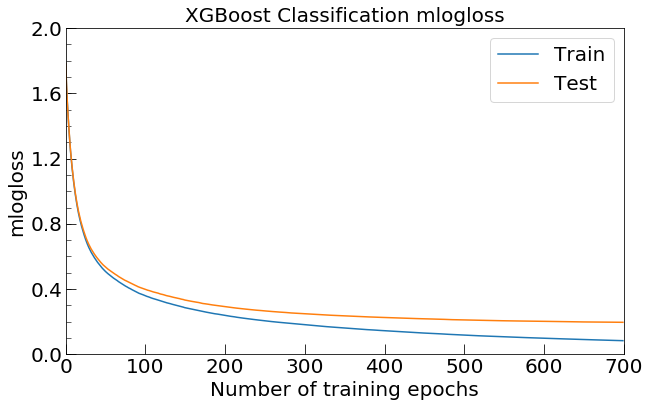
\includegraphics[scale=0.5]{./figs/xgb_epoch.png}
   
  \end{frame}


  
\end{document}